\pdfbookmark{Общая характеристика работы}{characteristic}             % Закладка pdf
\section*{Общая характеристика работы}

\newcommand{\actuality}{\pdfbookmark[1]{Актуальность}{actuality}\underline{\textbf{\actualityTXT}}}
\newcommand{\progress}{\pdfbookmark[1]{Разработанность темы}{progress}\underline{\textbf{\progressTXT}}}
\newcommand{\aim}{\pdfbookmark[1]{Цели}{aim}\underline{{\textbf\aimTXT}}}
\newcommand{\tasks}{\pdfbookmark[1]{Задачи}{tasks}\underline{\textbf{\tasksTXT}}}
\newcommand{\aimtasks}{\pdfbookmark[1]{Цели и задачи}{aimtasks}\aimtasksTXT}
\newcommand{\novelty}{\pdfbookmark[1]{Научная новизна}{novelty}\underline{\textbf{\noveltyTXT}}}
\newcommand{\influence}{\pdfbookmark[1]{Практическая значимость}{influence}\underline{\textbf{\influenceTXT}}}
\newcommand{\methods}{\pdfbookmark[1]{Методология и методы исследования}{methods}\underline{\textbf{\methodsTXT}}}
\newcommand{\defpositions}{\pdfbookmark[1]{Положения, выносимые на защиту}{defpositions}\underline{\textbf{\defpositionsTXT}}}
\newcommand{\reliability}{\pdfbookmark[1]{Достоверность}{reliability}\underline{\textbf{\reliabilityTXT}}}
\newcommand{\probation}{\pdfbookmark[1]{Апробация}{probation}\underline{\textbf{\probationTXT}}}
\newcommand{\contribution}{\pdfbookmark[1]{Личный вклад}{contribution}\underline{\textbf{\contributionTXT}}}
\newcommand{\publications}{\pdfbookmark[1]{Публикации}{publications}\underline{\textbf{\publicationsTXT}}}


Изучение явлений порядок-беспорядок --- фундаментальная задача равновесной статистической механики. Были приложены большие усилия, чтобы понять основные механизмы, ответственные за спонтанное упорядочение, а также природу фазовых переходов во многих типах систем. В частности, в течение последних лет большое внимание уделялось фрустрированным моделям~\cite{liebmann1986}. Термин «фрустрация» был введен~\cite{toulouse1977,vannimenus1977} для описания ситуации, когда спин (или количество спинов) в системе не может найти конфигурацию, полностью удовлетворяющей всем взаимодействиям с соседними спинами. Этот определение может быть применено к модели Изинга, моделям Поттса и векторным спинам. Как правило, фрустрация вызвана либо конкурирующими взаимодействиями или же решеточной структурой, как в треугольной, гранецентрированной кубической (ГЦК) и гексагонально-плотноупакованной (ГПУ) решетках с антиферромагнитным взаимодействием ближайших соседей. Фрустрационные эффекты чрезвычайно богаты, многие из которых в настоящее время еще не изучены.

Помимо того, что настоящие магнитные материалы с фрустрациями не поддаются точным решениям из-за нескольких видов взаимодействий, фрустрированные спиновые системы имеют свой собственный интерес в статистической механике. Недавние исследования показывают, что многие известные статистические методы и теории столкнулись со многими трудностями при работе с фрустрированными системами. В некотором смысле фрустрированные системы - отличные кандидаты для тестирования приближений и улучшения теории. Поскольку механизмы многих явлений не поняты в реальных системах (неупорядоченные системы, системы с дальним взаимодействием, трехмерные системы и т.д.), то стоит искать истоки этих явлений в точно решаемых системах. Эти точные результаты помогут качественно понять поведение реальных систем, которые в целом намного сложнее.
Однако, далеко не каждая физическая задача может быть решена точно. Такая ситуация скорее является исключением из правил, поскольку точное решение задачи связано с большим количеством сложных математических препятствий, которые чаще всего преодолеть не представляется возможным. Зачастую задачи такого типа решаются применением тех или иных приближений, которые значительно упрощают рассматриваемую задачу. Однако за этим упрощением стоит потеря значимой для исследователя информации.

Модель Изинга является простейшей задачей теории ферромагнетизма, решение которой в одномерном и двумерном случае можно получить точно~\cite{baxter1985}. Решение одномерной модели Изинга получил сам Изинг еще в 1925 году~\cite{ising1925}. Решению модели на двумерных решетках послужило опубликование Крамерсом и Ваннье статей~\cite{kramers_wannier1, kramers_wannier2}, в которых вводится так называемая трансфер-матрица. С помощью трансфер-матрицы авторы сначала переполучили результат Изинга на одномерной цепочке, после чего получили точное выражение для температуры фазового перехода на квадратной решетке. Впоследствии, этим результатом воспользовался Онзагер в 1941 году для получения точного решения модели Изинга на квадратной решетке~\cite{onsager1941}, которое, в свою очередь, привело к получению решений на других решетках (треугольная решетка --- Ваннье~\cite{wannier1950}, гексагональная решетка --- Гутаппель~\cite{houtapell1950}, кагоме --- Кано и Найя~\cite{kano_naya1953}), а также бурному развитию физики критических явлений~\cite{yang1952, brush1967, mussardo2010}. 

Труднопреодолимость весьма сложного оригинального метода Онзагера, а, главное, выдающийся результат Онзагера побудил многих высококлассных исследователей, как физиков, так и математиков, к поискам самых разнообразных направлений обобщений по разработке более простых и эффективных методов получения точных решений с одной стороны, а с другой стороны, к расширению объектов и задач исследований. Точное аналитическое решение для свободной энергии Гельмгольца в модели Изинга на квадратной решетке было успешно переполучено в разнообразных комбинаторных подходах, развитых, в частности, Кацем и Вардом~\cite{kac1952}, Поттсом и Вардом~\cite{potts1955}, Хёрстом и Грином~\cite{hurst1960}, Вдовиченко~\cite{vdovichenko1965_1, vdovichenko1965_2}, Фейнманом~\cite{feynmann1972}, а в более поздних теориях, основанных на грассмановых переменных: Самуэлем~\cite{samuel1980}, Плечко~\cite{plechko1985}, а также с использованием алгебры Клиффорда-Дирака Вергелесом~\cite{vergeles2009}.

К настоящему времени, количество научных статей по модели Изинга исчисляется тысячами и тысячами, и продолжает только увеличиваться, не обнаруживая спада активности. Однако следует отметить, что, несмотря на огромные затраченные усилия, направленные на поиски точных решений для свободной энергии в ряде случаев оказались не решенными до сих пор. Во-первых, это невозможность обобщения на 3D объекты. Во-вторых, отсутствие решений во внешнем магнитном поле ни на одной из 2D решеток. В-третьих, точно установлено, что решениям поддаются не все 2D решетки, а только лишь планарные, то есть те, в которых отсутствуют пересечения между обменными взаимодействиями. В-четвертых, модель Изинга при обобщении на спины с числом состояний более двух также не поддается точному решению. 

Ввиду указанных непреодолимых препятствий на пути более углубленных исследований, интересы исследователей постепенно переключались на применение модели Изинга к более широким объектам, в частности, 2D планарным решеткам: к классу одиннадцати Архимедовых и классу дуальных Архимедовым восьми решеток Лавэ; подробное изложение свойств решеток этих классов и строгое доказательство их уникальности изложено в книге Грюнбаума и Шефарда~\cite{grunbaum1987}. 

К настоящему времени точные выводы свободной энергии Гельмгольца получены на многих Архимедовых  решетках, а также некоторых решетках Лавэ (которые являются дуальными Архимедовым решеткам).

Поскольку точному решению поддаются только планарные решетки, а даже учет взаимодействия между спинами на вторых соседях не отвечает условию планарности, то интерес исследователей переключился на новое направление, а именно, возникли множественные попытки решить задачу в случае только взаимодействий между ближайшими соседями, но разных между разными соседними спинами. Фактически это означает переход на более высокий уровень — исследование решеток с трансляциями на два периода решетки по всем направлениям. Строго говоря, на всех указанных выше решетках такая задача решается как бы компромиссным образом — число учитываемых взаимодействий больше, чем с трансляциями на один период решетки, но меньше, чем на два периода. 

Так или иначе, была предпринята лишь одна попытка обобщения модели Изинга на две трансляции решетки, причем без какого либо вывода и исследования свойств полученного выражения, (см., например,~\cite{utiyama1951, syozi1972}).

В настоящей работе предлагается рассмотреть обобщенную модель Изинга сначала на одномерной цепочке с произвольным количеством различных обменных взаимодействий между спинами с учетом декорирования и магнитного поля, используя метод трансфер-матрицы Крамерса--Ваннье, а затем будет рассмотрена обобщенная модель Изинга на квадратной решетке с двумя различными обменными взаимодействиями решетки как в горизонтальном, так и вертикальном направлениях с учетом декорирования, но в отсутствие магнитного поля.

Необходимо отметить, что модель Изинга, как и любая другая математическая модель не привязана к какому-то конкретному материалу, соединению или эксперименту. К основным задачам таких моделей относятся выявление общих закономерностей в рассматриваемых процессах и явлениях, использование их в качестве прототипных для реальных трехмерных объектов и отклонение ложных догадок, сделанных на основе приближенных методов и экспериментальных результатов. 

{\actuality}\newline\indent
Экспериментальный материал по магнитным и термодинамическим свойствам фрустрированных соединений весьма богат. Однако, надлежащая интерпретация и теоретическое объяснение очень многих экспериментальных фактов в настоящее время отсутствует. Рассмотрение обобщенной модели Изинга позволит установить новые фрустрационные особенности, обусловленные наличием большого количества конкурирующих взаимодействий, а также позволит лучше понять свойства фрустрированных спиновых систем.

{\progress}\newline\indent
Несмотря на большое разнообразие всевозможных обобщений модели Изинга (например, модели Поттса, модель Гейзенберга и т.д.), не охвачен целый ряд задач, связанный с обобщением на произвольное число трансляций не только на линейной цепочке, но и на двумерных решетках. Привлекательность данного вида обобщения заключается в том, что такие задачи можно решать точно, не прибегая к различным приближениям.

{\aim} данной работы заключается в рассмотрении обобщенной модели Изинга с различными обменными взаимодействиями как между ближайшими, так и между вторыми соседями на одномерной цепочке с учетом декорирования и магнитного поля, а также на декорированных двумерных решетках, но в отсутствие поля, с последующим изучением их термодинамических, магнитных и фрустрационных свойств.

Для достижения цели были поставлены следующие {\tasks}:
\begin{enumerate}[beginpenalty=10000] % https://tex.stackexchange.com/a/476052/104425
  \item Получить точное аналитическое решение обобщенной модели Изинга на одномерной цепочке при учете магнитного поля методом трансфер-матрицы Крамерса--Ваннье;
  \item Исследовать термодинамические, магнитные и фрустрационные свойства обобщенной модели Изинга на одномерной цепочке, в том числе при учете декорирования; 
  \item Получить точное аналитическое решение обобщенной модели Изинга на квадратной решетке комбинаторным методом Вдовиченко--Фейнмана;
  \item Исследовать термодинамические и фрустрационные свойства обобщенной модели Изинга на квадратной решетке, в том числе при учете декорирования, но в отсутствие магнитного поля.
\end{enumerate}

{\novelty}
\begin{enumerate}[beginpenalty=10000] % https://tex.stackexchange.com/a/476052/104425 
  \item Впервые выведено точное выражение для свободной энергии Гельмгольца обобщенной модели Изинга на одномерной решетке с трансляциями на произвольное число периодов решетки;
  \item Впервые получено точное решение модели Изинга в магнитном поле на декорированной 1D цепочке с двумя трансляциями решетки;
  \item Комбинаторным методом Вдовиченко--Фейнмана были получены решения не только обобщенной модели Изинга на квадратной решетке, но и обычной модели Изинга на треугольной и гексагональной решетках;
  \item Исследованы термодинамические, магнитные и фрустрационные свойства обобщенной модели Изинга на одномерной цепочке и на декорированной цепочке;
  \item Изучены термодинамические и фрустрационные свойства обобщенной модели Изинга на квадратной решетке;
  \item Получены точные выражения для нуль-температурных энтропий и намагниченностей рассматриваемых моделей.
\end{enumerate}

{\influence} данной работы заключается в том, что полученные результаты могут быть использованы в качестве прототипных для изучения не только одномерных, но и 2D и 3D фрустрированных спиновых систем, а также в возможности рассмотрения широкого разнообразия физических свойств в решетках с различным декорированием. Стоит подчеркнуть, что подавляющее большинство реальных решеток являются декорированными. Более того, некоторые кристаллические решетки можно назвать декорированными, а именно, решетки ГЦК и ОЦК, в сравнении с простой кубической решеткой (ОЦК декорирована по объему куба, а ГЦК декорирована по шести граням куба).

{\methods}
\begin{enumerate}[beginpenalty=10000] 
  \item Метод трансфер-матрицы Крамерса--Ваннье;
  \item Комбинаторный метод Вдовиченко--Фейнмана.
\end{enumerate}

{\defpositions}
\begin{enumerate}[beginpenalty=10000] % https://tex.stackexchange.com/a/476052/104425
  \item Выведена трансфер-матрица Крамерса–Ваннье, обобщенная на произвольное число трансляций решетки, являющаяся произведением трансфер-матриц с одной трансляцией;
  \item Выведено точное аналитическое выражение для свободной энергии Гельмгольца обобщенной модели Изинга на квадратной решетке с двумя трансляциями с применением комбинаторного метода Вдовиченко-Фейнмана.
  \item Доказано, что промежуточные плато намагниченности в антиферромагнитной модели Изинга на декорированной решетке всегда представляются рациональными дробями $1/(d + 1)$ и $d/(d + 1)$, где $d$ --- произвольная степень декорирования;
  \item При увеличении степени декорирования ($d \rightarrow \infty$) влияние нодальных спинов становится все меньше и меньше, как в одномерной цепочке, так и в квадратной решетке, причем в последнем случае возникает квазиодномерное поведение;
  \item При исследовании фрустрированных систем получен вывод о том, что истинное поведение системы достигается только при комплексном исследовании, а исследование ограниченного числа наблюдаемых приводит к ошибочным результатам;
  \item Доказано, что значения нуль-температурных энтропий и намагниченностей в модели Изинга могут быть выражены через пределы некоторых целочисленных последовательностей;
  \item Выведено, что найденные значения нуль-температурных энтропий и намагниченностей на планарных решетках выражаются через математические сечения и математические константы, известные из теории чисел (золотое сечение, серебряное сечение, сверхзолотое сечение, пластическое число, постоянная Каталана, функция Клаузена). 
\end{enumerate}

{\reliability} полученных результатов обеспечивается строгой обоснованностью принятых приближений и допущений, использованием широко разработанных и обоснованных в мировой литературе аналитических и численных методов, а также тем фактом, что результаты находятся в согласии с теоретическими и экспериментальными работами других авторов.

{\probation}
Основные результаты работы докладывались на международных конференциях, семинарах и симпозиумах:
\begin{enumerate} [beginpenalty=10000]
	\item VII Euro-Asian Symposium «Trends in MAGnetism», 8--13 сентября 2019 года, Екатеринбург.
	\item XIII Международный семинар молодых ученых «Магнитные фазовые переходы»; 17 сентября 2019 года, Махачкала.
	\item Международная зимняя школа физиков-теоретиков «Коуровка–XXXVIII», 23--29 февраля 2020 года, «Гранатовая бухта», Верхняя Сысерть.
	\item 54-я Школа ПИЯФ по Физике Конденсированного Состояния (Школа ФКС-2020), 16--21 марта 2020 года, Гатчина:НИЦ «Курчатовский институт», Санкт-Петербург.
	\item VII Международная молодежная научная конференция Физика. Технологии. Инновации ФТИ-2020; 18--22 мая 2020 года, Екатеринбург.
	\item VIII Международная молодежная научная конференция Физика. Технологии. Инновации ФТИ-2021; 17--21 мая 2021 года, Екатеринбург.
	\item Забабахинские научные чтения 2021, 27 сентября -- 01 октября 2021 года, Снежинск.
	\item Молодежная школа по физике конденсированного состояния (Школа ФКС-2024), 11--15 марта 2024 года, База отдыха «Лосево Парк», Ленинградская область.
\end{enumerate}

{\contribution} Автор самостоятельно проводил поиск и анализ научной литературы по теме работы, под руководством научного руководителя выполнял задачи, поставленные в начале работы над диссертацией, участвовал в получении и обсуждении ряда результатов, написании тезисов и статей.

\ifnumequal{\value{bibliosel}}{0}
{%%% Встроенная реализация с загрузкой файла через движок bibtex8. (При желании, внутри можно использовать обычные ссылки, наподобие `\cite{vakbib1,vakbib2}`).
    {\publications} Основные результаты по теме диссертации изложены
    в~XX~печатных изданиях,
    X из которых изданы в журналах, рекомендованных ВАК,
    X "--- в тезисах докладов.
}%
{%%% Реализация пакетом biblatex через движок biber
    \begin{refsection}[bl-author, bl-registered]
        % Это refsection=1.
        % Процитированные здесь работы:
        %  * подсчитываются, для автоматического составления фразы "Основные результаты ..."
        %  * попадают в авторскую библиографию, при usefootcite==0 и стиле `\insertbiblioauthor` или `\insertbiblioauthorgrouped`
        %  * нумеруются там в зависимости от порядка команд `\printbibliography` в этом разделе.
        %  * при использовании `\insertbiblioauthorgrouped`, порядок команд `\printbibliography` в нём должен быть тем же (см. biblio/biblatex.tex)
        %
        % Невидимый библиографический список для подсчёта количества публикаций:
        \phantom{\printbibliography[heading=nobibheading, section=1, env=countauthorvak,          keyword=biblioauthorvak]%
        \printbibliography[heading=nobibheading, section=1, env=countauthorwos,          keyword=biblioauthorwos]%
        \printbibliography[heading=nobibheading, section=1, env=countauthorscopus,       keyword=biblioauthorscopus]%
        \printbibliography[heading=nobibheading, section=1, env=countauthorconf,         keyword=biblioauthorconf]%
        \printbibliography[heading=nobibheading, section=1, env=countauthorother,        keyword=biblioauthorother]%
        \printbibliography[heading=nobibheading, section=1, env=countregistered,         keyword=biblioregistered]%
        \printbibliography[heading=nobibheading, section=1, env=countauthorpatent,       keyword=biblioauthorpatent]%
        \printbibliography[heading=nobibheading, section=1, env=countauthorprogram,      keyword=biblioauthorprogram]%
        \printbibliography[heading=nobibheading, section=1, env=countauthor,             keyword=biblioauthor]%
        \printbibliography[heading=nobibheading, section=1, env=countauthorvakscopuswos, filter=vakscopuswos]%
        \printbibliography[heading=nobibheading, section=1, env=countauthorscopuswos,    filter=scopuswos]}%
        %
        \nocite{*}%
        %
        {\publications} Основные результаты по теме диссертации изложены в~\arabic{citeauthor}~печатных изданиях,
        \arabic{citeauthorvak} из которых изданы в журналах, рекомендованных ВАК%
        \ifnum \value{citeauthorscopuswos}>0%
            , \arabic{citeauthorscopuswos} "--- в~периодических научных журналах, индексируемых Web of~Science и Scopus%
        \fi%
        \ifnum \value{citeauthorconf}>0%
            , \arabic{citeauthorconf} "--- в~тезисах докладов.
        \else%
            .
        \fi%
%        \ifnum \value{citeregistered}=0%
%            \ifnum \value{citeauthorpatent}=0%
%                Зарегистрирован \arabic{citeauthorpatent} патент.
%            \fi%
%            \ifnum \value{citeauthorprogram}=0%
%                Зарегистрирована \arabic{citeauthorprogram} программа для ЭВМ.
%            \fi%
%        \fi%
%        \ifnum \value{citeregistered}>1%
%            Зарегистрированы\ %
%            \ifnum \value{citeauthorpatent}>0%
%            \formbytotal{citeauthorpatent}{патент}{}{а}{}%
%            \ifnum \value{citeauthorprogram}=0 . \else \ и~\fi%
%            \fi%
%            \ifnum \value{citeauthorprogram}>0%
%            \formbytotal{citeauthorprogram}{программ}{а}{ы}{} для ЭВМ.
%            \fi%
%        \fi%
        % К публикациям, в которых излагаются основные научные результаты диссертации на соискание учёной
        % степени, в рецензируемых изданиях приравниваются патенты на изобретения, патенты (свидетельства) на
        % полезную модель, патенты на промышленный образец, патенты на селекционные достижения, свидетельства
        % на программу для электронных вычислительных машин, базу данных, топологию интегральных микросхем,
        % зарегистрированные в установленном порядке.(в ред. Постановления Правительства РФ от 21.04.2016 N 335)
    \end{refsection}%
    \begin{refsection}[bl-author, bl-registered]
        % Это refsection=2.
        % Процитированные здесь работы:
        %  * попадают в авторскую библиографию, при usefootcite==0 и стиле `\insertbiblioauthorimportant`.
        %  * ни на что не влияют в противном случае
        \nocite{vakbib2}%vak
        \nocite{patbib1}%patent
        \nocite{progbib1}%program
        \nocite{bib1}%other
        \nocite{confbib1}%conf
    \end{refsection}%
        %
        % Всё, что вне этих двух refsection, это refsection=0,
        %  * для диссертации - это нормальные ссылки, попадающие в обычную библиографию
        %  * для автореферата:
        %     * при usefootcite==0, ссылка корректно сработает только для источника из `external.bib`. Для своих работ --- напечатает "[0]" (и даже Warning не вылезет).
        %     * при usefootcite==1, ссылка сработает нормально. В авторской библиографии будут только процитированные в refsection=0 работы.
}

%При использовании пакета \verb!biblatex! будут подсчитаны все работы, добавленные
%в файл \verb!biblio/author.bib!. Для правильного подсчёта работ в~различных
%системах цитирования требуется использовать поля:
%\begin{itemize}
%        \item \texttt{authorvak} если публикация индексирована ВАК,
%        \item \texttt{authorscopus} если публикация индексирована Scopus,
%        \item \texttt{authorwos} если публикация индексирована Web of Science,
%        \item \texttt{authorconf} для докладов конференций,
%        \item \texttt{authorpatent} для патентов,
%        \item \texttt{authorprogram} для зарегистрированных программ для ЭВМ,
%        \item \texttt{authorother} для других публикаций.
%\end{itemize}
%Для подсчёта используются счётчики:
%\begin{itemize}
%        \item \texttt{citeauthorvak} для работ, индексируемых ВАК,
%        \item \texttt{citeauthorscopus} для работ, индексируемых Scopus,
%        \item \texttt{citeauthorwos} для работ, индексируемых Web of Science,
%        \item \texttt{citeauthorvakscopuswos} для работ, индексируемых одной из трёх баз,
%        \item \texttt{citeauthorscopuswos} для работ, индексируемых Scopus или Web of~Science,
%        \item \texttt{citeauthorconf} для докладов на конференциях,
%        \item \texttt{citeauthorother} для остальных работ,
%        \item \texttt{citeauthorpatent} для патентов,
%        \item \texttt{citeauthorprogram} для зарегистрированных программ для ЭВМ,
%        \item \texttt{citeauthor} для суммарного количества работ.
%\end{itemize}
% Счётчик \texttt{citeexternal} используется для подсчёта процитированных публикаций;
% \texttt{citeregistered} "--- для подсчёта суммарного количества патентов и программ для ЭВМ.

%Для добавления в список публикаций автора работ, которые не были процитированы в
%автореферате, требуется их~перечислить с использованием команды \verb!\nocite! в
%\verb!Synopsis/content.tex!.
 % Характеристика работы по структуре во введении и в автореферате не отличается (ГОСТ Р 7.0.11, пункты 5.3.1 и 9.2.1), потому её загружаем из одного и того же внешнего файла, предварительно задав форму выделения некоторым параметрам

%Диссертационная работа была выполнена при поддержке грантов \dots

%\underline{\textbf{Объем и структура работы.}} Диссертация состоит из~введения,
%четырех глав, заключения и~приложения. Полный объем диссертации
%\textbf{ХХХ}~страниц текста с~\textbf{ХХ}~рисунками и~5~таблицами. Список
%литературы содержит \textbf{ХХX}~наименование.

\pdfbookmark{Содержание работы}{description}                          % Закладка pdf
\section*{Содержание работы}
Во \underline{\textbf{введении}} обосновывается актуальность
исследований, проводимых в~рамках данной диссертационной работы,
приводится обзор научной литературы по~изучаемой проблеме,
формулируется цель, ставятся задачи работы, излагается научная новизна
и практическая значимость представляемой работы. В~последующих главах
сначала описывается общий принцип, позволяющий \dots, а~потом идёт
апробация на частных примерах: \dots  и~\dots.


\underline{\textbf{Первая глава}} посвящена \dots

картинку можно добавить так:
\begin{figure}[ht]
    \centerfloat{
        \hfill
        \subcaptionbox{\LaTeX}{%
            
\includegraphics[scale=0.27]{latex}}
        \hfill
        \subcaptionbox{Knuth}{%
            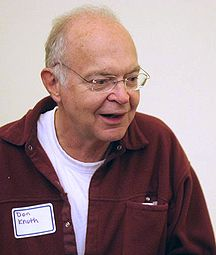
\includegraphics[width=0.25\linewidth]{knuth1}}
        \hfill
    }
    \caption{Подпись к картинке.}\label{fig:latex}
\end{figure}

Формулы в строку без номера добавляются так:
\[
    \lambda_{T_s} = K_x\frac{d{x}}{d{T_s}}, \qquad
    \lambda_{q_s} = K_x\frac{d{x}}{d{q_s}},
\]

\underline{\textbf{Вторая глава}} посвящена исследованию

\underline{\textbf{Третья глава}} посвящена исследованию

Можно сослаться на свои работы в автореферате. Для этого в файле
\verb!Synopsis/setup.tex! необходимо присвоить положительное значение
счётчику \verb!\setcounter{usefootcite}{1}!. В таком случае ссылки на
работы других авторов будут подстрочными.
Изложенные в третьей главе результаты опубликованы в~\cite{vakbib1, vakbib2}.
Использование подстрочных ссылок внутри таблиц может вызывать проблемы.

В \underline{\textbf{четвертой главе}} приведено описание

\FloatBarrier
\pdfbookmark{Заключение}{conclusion}                                  % Закладка pdf
В \underline{\textbf{заключении}} приведены основные результаты работы, которые заключаются в следующем:
%% Согласно ГОСТ Р 7.0.11-2011:
%% 5.3.3 В заключении диссертации излагают итоги выполненного исследования, рекомендации, перспективы дальнейшей разработки темы.
%% 9.2.3 В заключении автореферата диссертации излагают итоги данного исследования, рекомендации и перспективы дальнейшей разработки темы.
\begin{enumerate}
  \item На основе анализа \ldots
  \item Численные исследования показали, что \ldots
  \item Математическое моделирование показало \ldots
  \item Для выполнения поставленных задач был создан \ldots
\end{enumerate}


\pdfbookmark{Литература}{bibliography}                                % Закладка pdf
При использовании пакета \verb!biblatex! список публикаций автора по теме
диссертации формируется в разделе <<\publications>>\ файла
\verb!common/characteristic.tex!  при помощи команды \verb!\nocite!

\ifdefmacro{\microtypesetup}{\microtypesetup{protrusion=false}}{} % не рекомендуется применять пакет микротипографики к автоматически генерируемому списку литературы
\urlstyle{rm}                               % ссылки URL обычным шрифтом
\ifnumequal{\value{bibliosel}}{0}{% Встроенная реализация с загрузкой файла через движок bibtex8
    \renewcommand{\bibname}{\large \bibtitleauthor}
    \nocite{*}
    \insertbiblioauthor           % Подключаем Bib-базы
    %\insertbiblioexternal   % !!! bibtex не умеет работать с несколькими библиографиями !!!
}{% Реализация пакетом biblatex через движок biber
    % Цитирования.
    %  * Порядок перечисления определяет порядок в библиографии (только внутри подраздела, если `\insertbiblioauthorgrouped`).
    %  * Если не соблюдать порядок "как для \printbibliography", нумерация в `\insertbiblioauthor` будет кривой.
    %  * Если цитировать каждый источник отдельной командой --- найти некоторые ошибки будет проще.
    %
    %% authorvak
    \nocite{vakbib1}%
    \nocite{vakbib2}%
    \nocite{vakbib3}%
    \nocite{vakbib4}%
    \nocite{vakbib5}%
    \nocite{vakbib6}%
    \nocite{vakbib7}%
    \nocite{vakbib8}%
    \nocite{vakbib9}%
    \nocite{vakbib10}%
    \nocite{vakbib11}%
    \nocite{vakbib12}%
    %
    %% authorwos
    \nocite{wosbib1}%
    %
    %% authorscopus
    \nocite{scbib1}%
    %
    %% authorpatent
    \nocite{patbib1}%
    %
    %% authorprogram
    \nocite{progbib1}%
    %
    %% authorconf
    \nocite{confbib1}%
    \nocite{confbib2}%
    %
    %% authorother
    \nocite{bib1}%
    \nocite{bib2}%

    \ifnumgreater{\value{usefootcite}}{0}{
        \begin{refcontext}[labelprefix={}]
            \ifnum \value{bibgrouped}>0
                \insertbiblioauthorgrouped    % Вывод всех работ автора, сгруппированных по источникам
            \else
                \insertbiblioauthor      % Вывод всех работ автора
            \fi
        \end{refcontext}
    }{
        \ifnum \totvalue{citeexternal}>0
            \begin{refcontext}[labelprefix=A]
                \ifnum \value{bibgrouped}>0
                    \insertbiblioauthorgrouped    % Вывод всех работ автора, сгруппированных по источникам
                \else
                    \insertbiblioauthor      % Вывод всех работ автора
                \fi
            \end{refcontext}
        \else
            \ifnum \value{bibgrouped}>0
                \insertbiblioauthorgrouped    % Вывод всех работ автора, сгруппированных по источникам
            \else
                \insertbiblioauthor      % Вывод всех работ автора
            \fi
        \fi
        %  \insertbiblioauthorimportant  % Вывод наиболее значимых работ автора (определяется в файле characteristic во второй section)
        \begin{refcontext}[labelprefix={}]
            \insertbiblioexternal            % Вывод списка литературы, на которую ссылались в тексте автореферата
        \end{refcontext}
        % Невидимый библиографический список для подсчёта количества внешних публикаций
        % Используется, чтобы убрать приставку "А" у работ автора, если в автореферате нет
        % цитирований внешних источников.
        \printbibliography[heading=nobibheading, section=0, env=countexternal, keyword=biblioexternal, resetnumbers=true]%
    }
}
\ifdefmacro{\microtypesetup}{\microtypesetup{protrusion=true}}{}
\urlstyle{tt}                               % возвращаем установки шрифта ссылок URL
